\section{Criação da biblioteca \textit{Last-Mile-Routing-Analyzer}} \label{BibLMRA}

Para realizar os dois estudos de casos de forma eficiente e replicável, foi desenvolvida e publicada uma biblioteca de código aberto escrita em linguagem \textit{Python}, nomeada \textit{lmr\_analyzer}.
%
Tal biblioteca consolida uma série de rotinas desenvolvidas durante o trabalho em prol de se obter conhecimentos relevantes a partir das bases de dados e informações geográficas disponibilizadas.
%
Todos os códigos estão disponíveis e documentados publicamente na plataforma Github (\citeauthoronline{guilherme_fernandes_alves_2022_6792977}, \citeyear{guilherme_fernandes_alves_2022_6792977}).
%
Os termos pacote, módulo e biblioteca são utilizados como sinônimos neste trabalho. 
Alguns conceitos de programação orientada a objetos (\citeauthoronline{cox1986object}, \citeyear{cox1986object}) serão empregados ao longo do texto, tais como classes, métodos, atributos, etc.. 

A estrutura básica do pacote \textit{lmr\_analyzer} pode ser vista na Figura \ref{fig:UMLPython}, de onde se obtém que as principais classes desenvolvidas são: \textit{package}, \textit{stop}, \textit{route}, \textit{distanceMatrix}, \textit{analysis} e \textit{geometry}, além de um módulo \textit{amzSerializer} específico para tratamento da base de dados da Amazon.
%
A classe \textit{package} é a primeira das classes básicas da \textit{lmr\_analyzer}, ela concentra as informações de dimensão e status de cada pacote a ser entregue, i.e. se ele se trata de um pacote entregue, devolvido ou a ser entregue.
%
A classe \textit{stop} armazena informações relativas aos diferentes pontos de interesse, sejam eles PDEs ou CDs.
%
Para ser inicializada, a classe \textit{stop} recebe um ou mais objetos da classe \textit{package}, além de informações como a latitude e longitude do local e os horários de funcionamento.
%
Em seguida, um conjunto de objetos da classe \textit{stop} é utilizado para definir um objeto da classe \textit{route} que, para que seja inicializado, também necessita de um objeto \textit{vehicle} e do horário de início da rota.
%
Finalmente, a classe \textit{analysis} realiza operações com base nos dados armazenados em um conjunto de \textit{routes} e um objeto \textit{geometry} que descreve as informações espaciais disponíveis.
%
Adicionalmente, o submódulo \textit{utils} contém funções e métodos genéricos que podem ser reutilizadas pelas demais classes.
%
Através dessa estrutura de dados é possível tirar proveito, simultaneamente, das informações espacial e das bases de dados fornecidas. 

\begin{figure}[H]
    \centering
    \caption{Diagrama UML da biblioteca \textit{lmr\_analyzer}}
    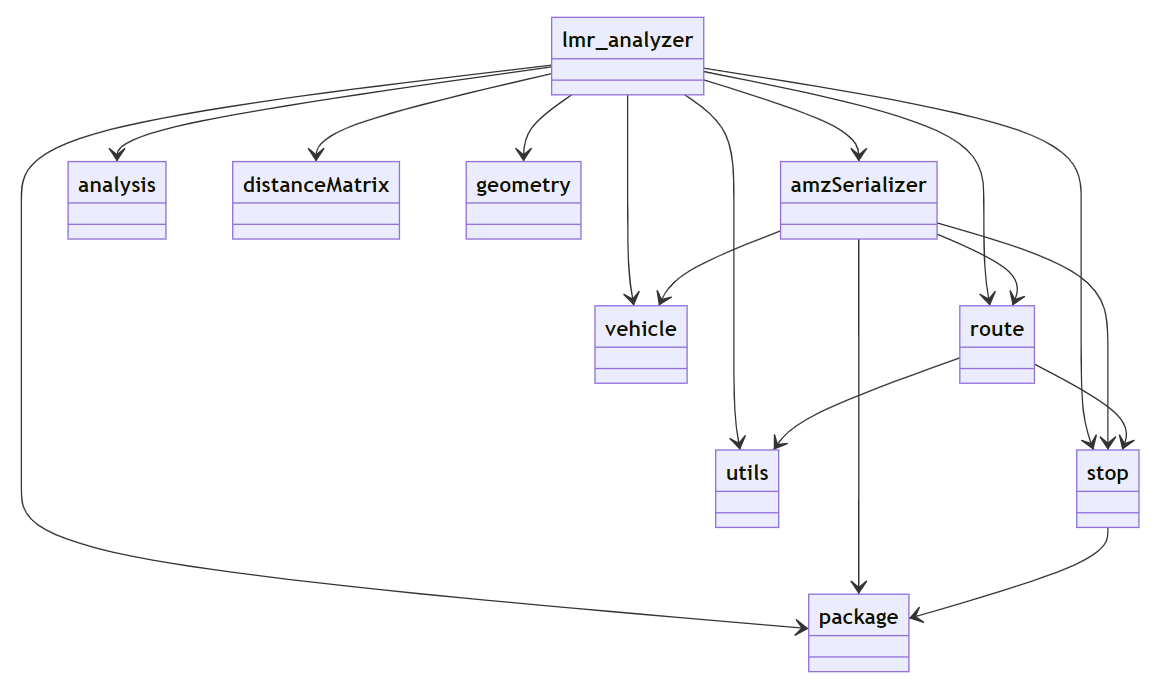
\includegraphics[width=0.6\textwidth]{images/4_materiais/lmr_analyzer/lmr_analyzer_UML.png}
    \caption*{Fonte: Produzido pelos autores Fernandes \& Alves}
    \label{fig:UMLPython}
\end{figure}

Dentre as funcionalidades disponíveis na \textit{lmr\_analyzer} estão a capacidade de processar e armazenar os dados de entregas última milha em objetos de diferentes classes, obtenção de distancias sob diferentes modos (euclidiana, distância veicular, etc.), cálculo de fator de circuito, análise quantitativa de malhas viárias incluindo distribuição da orientação de vias e, finalmente, a importação e exportação de arquivos \textit{shapefiles} contendo as informações analisadas.
%
Além disso, devido à flexibilidade da linguagem de programação \textit{Python}, é possível integrar os resultados e dados de entrada da biblioteca com as demais ferramentas do trabalho.
%
Na prática, o que se estabelece é um procedimento - \textit{framework} - que facilita a transformação de dados brutos em resultados tratados que podem ser visualizados em diversos ambientes, como por exemplo o \textit{QGIS}.
%
A seguir, apresenta-se detalhadamente cada uma das funcionalidades mencionadas. 
Contudo, destaca-se que um maior detalhamento de cada etapa está presente na seção de apêndice \ref{sec:AppCodes}.

\subsection{Fluxo de trabalho}

Explorando o tópico de flexibilidade como uma das vantagens da biblioteca criada, podemos descrever qual a usabilidade esperada ao se trabalhar com a mesma.
%
O fluxo de trabalho padrão estabelecido através da biblioteca acompanha o modelo descrito na Figura \ref{fig:flowchart}. 
%
Podemos notar que o usuário precisa primeiro definir o conjunto de dados relativos às rotas a serem analisadas.
%
Duas sequências podem ser atribuídas nesta etapa, com auxílio da classe \textit{route}, sendo elas a sequência programada e a sequencia realmente executada.
Essas duas sequências são completamente independentes, e o \textit{software} não requer que ambas sejam inseridas simultaneamente para que se obtenha os resultados disponíveis.
%
Em outras palavras, caso o usuário disponha apenas de informações relativas a rotas programadas, sem ter dados de como as rotas realmente se saíram na prática, poderá utilizar a ferramenta para realizar os estudos que serão indicados ao longo deste trabalho.
O caminho contrário também é possível.

Já quanto às informações espaciais, estas em geral representam dados não muito diferentes dos que foram apresentados na seção \ref{sec:dados_de_informacao_geografica}.
%
Em suma, um arquivo \textit{\textit{shapefile}} que contenha uma descrição espacial da cidade a ser analisada pode ser utilizado como dado de entrada.
%
Para as análises que serão feitas neste trabalho, escolheu-se uma discretização da cidade através dos contornos dos bairros.

\begin{figure}[H]
    \centering
    \caption{Fluxo de dados para utilização da biblioteca \textit{lmr\_analyzer}}
    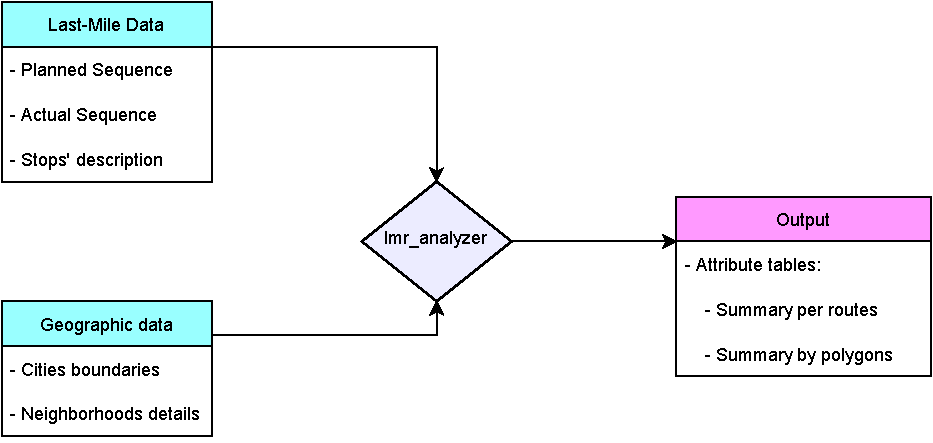
\includegraphics[width=0.8\textwidth]{images/4_materiais/lmr_analyzer/flowchart.pdf}
    \caption*{Fonte: Produzido pelos autores Fernandes \& Alves}
    \label{fig:flowchart}
\end{figure}


\subsection{Cálculo do fator de circuito através do \textit{Google Maps API}} \label{sec:codigosmaps}

Inicialmente foi utilizada a plataforma \textit{Google Maps} para cálculo das distâncias reais percorridas entre diferentes PDEs e o CD, para então compará-las com a distância euclidiana por meio da medida de fator de circuito introduzida no capítulo \ref{sec:revis_biblio}. 
%
O método utilizado para se obter as distâncias do \textit{Google Maps} através da \textit{lmr\_analyzer} estão descritos na subseção \ref{sec:codigosmaps}, no capítulo de apêndice \ref{sec:AppCodes}.
%
A partir da Figura \ref{fig:rota_LA_CF} podemos visualizar um exemplo comum de rotas que serão estudadas.
No caso em questão, as distâncias a serem calculadas estão representadas pelas linhas cheias, que correspondem com a sequência real que a rota apresentou.

\begin{figure}[htbp]
     \caption{Exemplo de rota na cidade de Los Angeles}
     \begin{subfigure}{.49\textwidth}
         \centering
         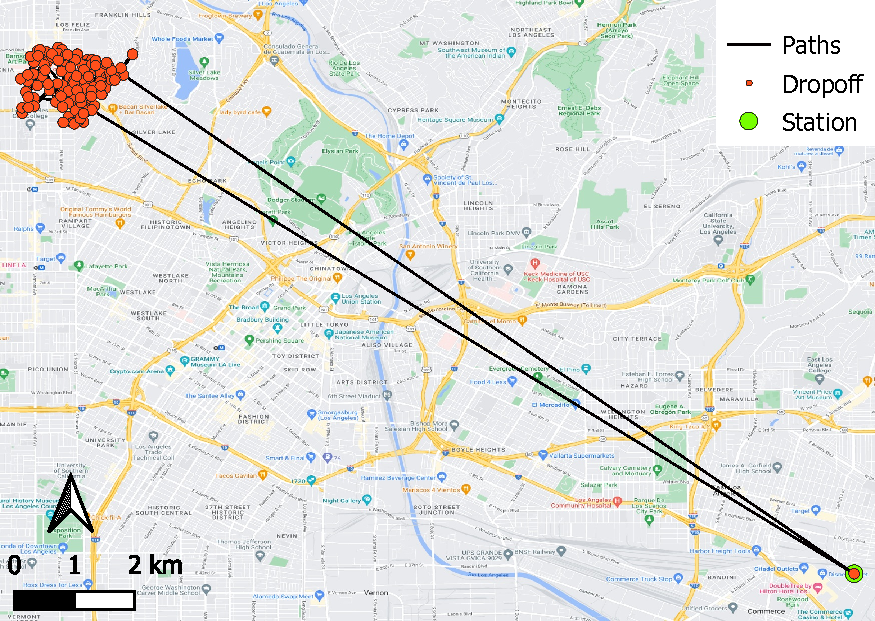
\includegraphics[height=0.63\textwidth]{images/4_materiais/lmr_analyzer/cf_LA_example_zoom.pdf}
     \end{subfigure}
     \begin{subfigure}{.49\textwidth}
       \centering
       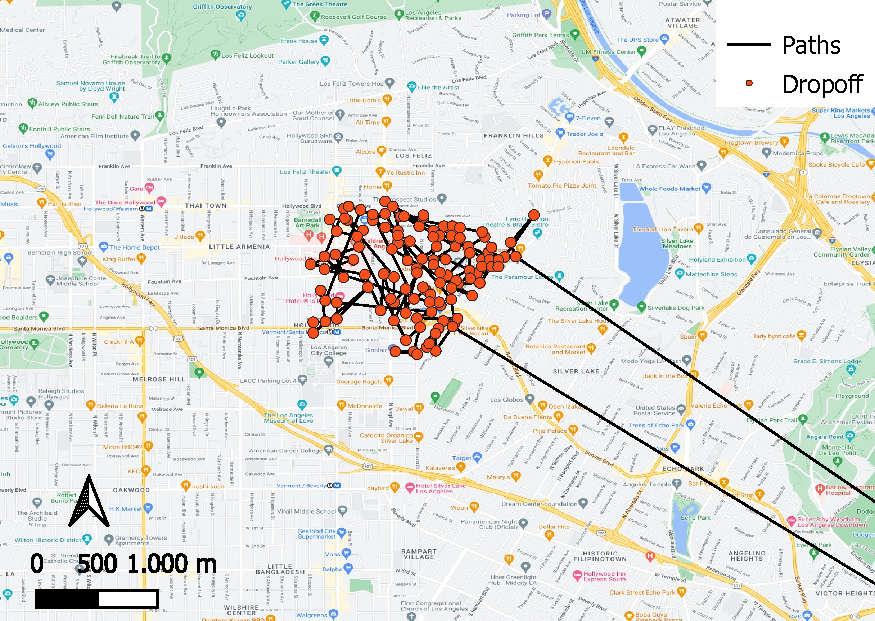
\includegraphics[height=0.63\textwidth]{images/4_materiais/lmr_analyzer/cf_LA_example_zoom_in.pdf}
     \end{subfigure}
     \caption*{\ Fonte: Produzido pelos autores Fernandes \& Alves}
     \label{fig:rota_LA_CF}
 \end{figure} % Repasses

Ademais, para complementar a análise também é preciso estimar a distância em linha reta entre os diferentes pontos.
%
Será adotada a aproximação de que as distâncias entre os pontos são sempre suficientemente pequenas, assim permitindo utilizar a fórmula de \textit{Haversine} (\citeauthoronline{robusto1957cosine}, \citeyear{robusto1957cosine}) para se obter a distância de grande círculo e então aproximá-la como sendo a distância euclidiana entre os pontos.
%
Como essas distâncias não passam de duas centenas de quilômetros, tal hipótese pode ser adotada sem grandes problemas.

Tendo posse da distância em linha reta e das distâncias veiculares (\textit{driving distances}), é possível calcular o fator de circuito entre os diferentes trechos de cada rota.
Ademais, calcula-se também o fator de circuito global de cada rota de acordo com a Equação \ref{eq:Cf_TOTAL}.

\begin{equation} \label{eq:Cf_TOTAL}
    CF_{total} = \frac{total\;driving\;distance}{total\;euclidean\;distance}
\end{equation}

Sendo assim, os atributos que serão calculados nesta etapa, portanto, são: 
\begin{enumerate}
    \item \textbf{planned\_driving\_distances}: Vetor contendo as distâncias reais percorridas entre cada trecho da rota. Este vetor contém $n$ elementos, sendo $n$ o número de entregas. Considera-se que, ao realizar a última entrega, o veículo retorna para o ponto de origem (geralmente o CD). Cada elemento do vetor representa a distância do PDE que está naquela posição até o PDE subsequente. 
    \item \textbf{planned\_euclidean\_distances}: Vetor análogo ao descrito imediatamente acima, porém desta vez contendo as distâncias em linha reta entre os diferentes PDEs.
    \item \textbf{planned\_circuity\_factors}: Representa o fator de circuito entre cada um dos trechos. É calculado simplesmente dividindo-se os dois vetores anteriores.
    \item \textbf{avg\_planned\_circuity\_factor}: Representa a média do fator de circuito dos trechos, os seja, a média do vetor planned\_circuity\_factors.
    \item \textbf{max\_planned\_circuity\_factor}: Valor máximo do fator de circuito da rota.
    \item \textbf{min\_planned\_circuity\_factor}: Valor mínimo do fator de circuito da rota.
    \item \textbf{total\_planned\_driving\_distance}: Soma de todas as distâncias percorridas na rota.
    \item \textbf{total\_planned\_euclidean\_distance}: Soma de todas as distâncias euclidianas.
    \item \textbf{total\_planned\_circuity\_factor}: Divisão entre a soma de distâncias percorridas e a soma de distâncias euclidianas. Representa a medida $CF_{total}$, tal como apresentada na Equação \ref{eq:Cf_TOTAL}.
\end{enumerate}

Estes atributos se repetem, da mesma forma, para a sequência real executada. 
As operações básicas entre os diferentes vetores (soma, divisão, etc.) são facilitadas através de programas escritos linguagem C e contidos na biblioteca \textit{numpy} para \textit{Python} (\citeauthoronline{harris2020array}, \citeyear{harris2020array}).

%%%%%%%%%%%%%%%%%%%%%%%%%%%%%%%%%%%%%%%%%%%%%%%%%%%%%%%%%%%%%%%%%
\subsection{\textit{OSRM} como alternativa ao \textit{Google Maps API}}

Um problema enfrentado na abordagem anterior é a limitação de número de consultas gratuitas permitidas pela \textit{API} do \textit{Google Maps}, o que exigiria investimento financeiro para finalizar a pesquisa (ou seja, para para utilizar a ferramenta acima de um certo limite).
Sendo assim, buscou-se como alternativa a plataforma \textit{Open Source Routing Machine} (\citeauthoronline{luxen2011real}, \citeyear{luxen2011real}), que permite calcular todas as possíveis rotas entre dois ou mais pontos diferentes e, assim, escolher a rota de menor caminho ou tempo.
%
A ferramenta recebe como dados de entrada as coordenadas geodésicas dos pontos a serem analisados e, como resultado, entrega a distância a ser percorrida, o tempo previsto de deslocamento e também o caminho a ser percorrido.
Para o trabalho em questão, apenas a distância será utilizada, aliviando a quantidade de dados a serem armazenados.
Uma descrição mais detalhada do método empregado encontra-se disponível na seção de apêndices \ref{sec:AppCodes}.

De toda forma, ambas as metodologias (\textit{googlemaps} e \textit{OSRM}) permanecem disponíveis na biblioteca \textit{lmr\_analyzer} e, dependendo da aplicação, o usuário final poderá escolher qual a mais adequada.
%
Para o desenvolvimento deste trabalho, algumas das distâncias foram calculadas utilizado o método do \textit{Google Maps}, uma vez que a plataforma oferece um período de utilização livre de cobranças (\textit{free trail}).
Uma vez encerrado este período, passou-se a utilizar a plataforma exclusivamente a plataforma \textit{open-source}.

%%%%%%%%%%%%%%%%%%%%%%%%%%%%%%%%%%%%%%%%%%%%%%%%%%%%%%%%%%%%%%%
\subsection{Modelo para avaliação topológica de malhas viárias}

Uma vez definidos os valores da medida de fator de circuito para cada trecho de rota, bem como para a rota como um todo, foi possível explorar a vertente geoespacial da análise, que neste caso é representada pela malha viária da cidade.
%
Para tanto, foi utilizada a biblioteca \textit{OSMnx} (\citeauthoronline{BOEING2017126}, \citeyear{BOEING2017126}) que, conforme descrito na seção \ref{sec:revis_biblio}, permite modelar, analisar e visualizar a estrutura de malhas viárias tomando como base dados disponíveis na plataforma do \textit{OpenStreetMap}.
%
A \textit{OSMnx} faz uso da biblioteca \textit{geopandas} (\citeauthoronline{jordahl2014geopandas}, \citeyear{jordahl2014geopandas}) para facilitar o tratamento de dados espaciais, assim, este trabalho também fez uso de tal biblioteca. 
O que foi realizado dentro do pacote \textit{lmr\_analyzer}, através de um arquivo em formato \textit{shapefile} que descreva o contorno de cada bairro da cidade, iterar sobre cada polígono e criar um grafo (\textit{graph}) contendo arcos e nós que representem a malha viária do bairro em questão.
A Figura \ref{fig:graphs_gru_example} apresenta um exemplo de alguns dos grafos gerados para a cidade de Guarulhos, onde os arcos representam segmentos de vias e os nós representam intersecções entre arcos ou extremidades de arcos.

\begin{figure}[htb]
    \centering
    \caption{Exemplo de grafo gerado com o \textit{osmnx} para o bairro de Cumbica em Guarulhos, SP}
        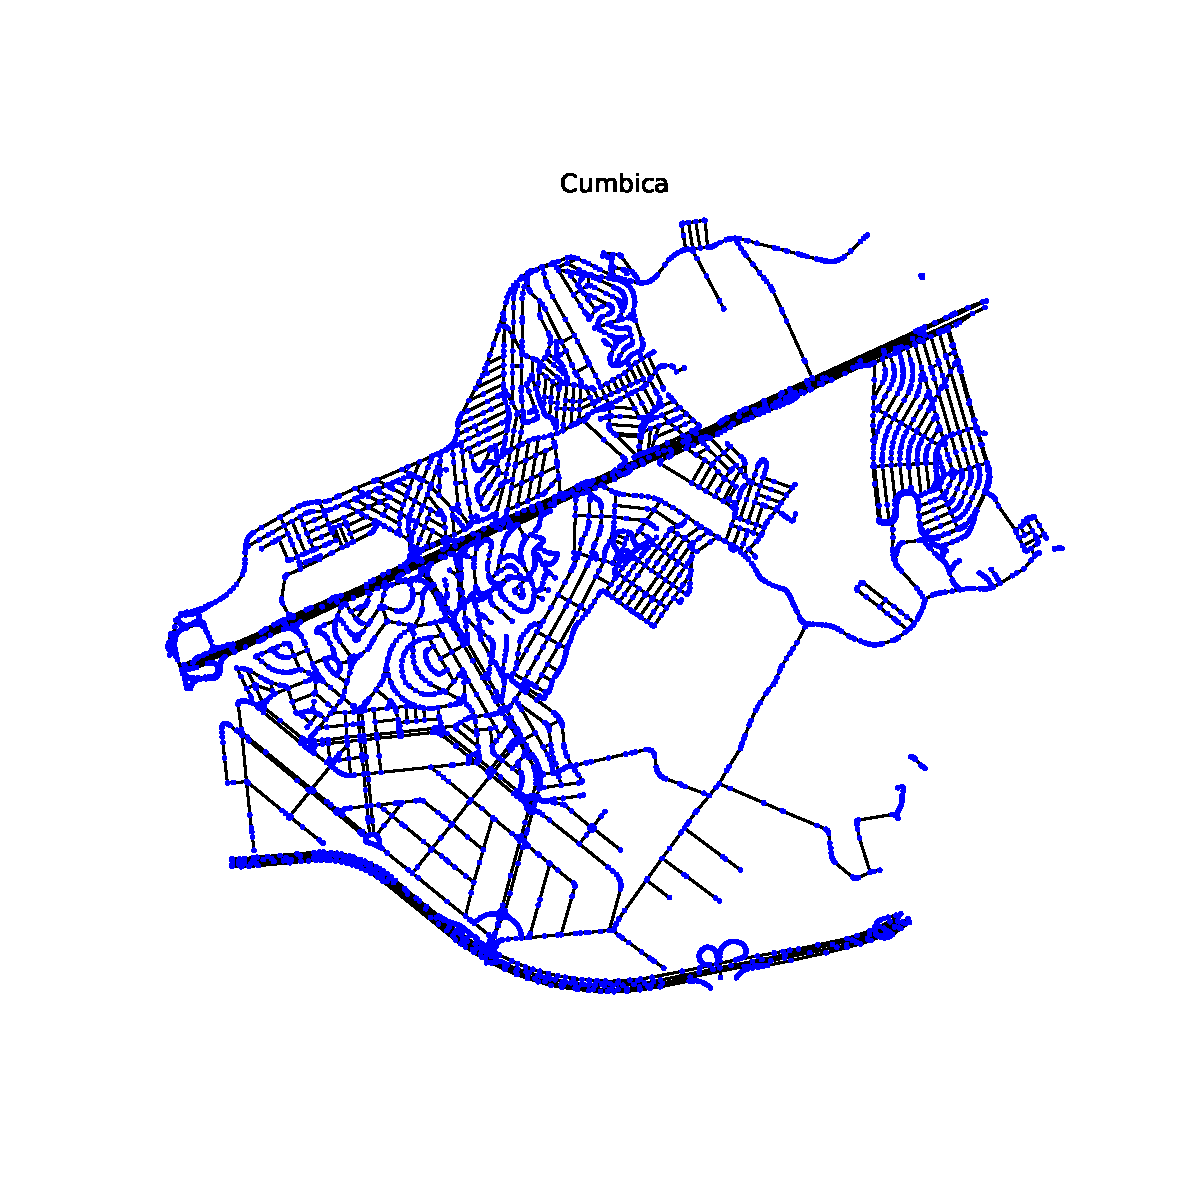
\includegraphics[width=0.6\linewidth]{images/4_materiais/lmr_analyzer/graph_Cumbica.pdf}
    \caption*{\ Fonte: Produzido pelos autores Fernandes \& Alves}
    \label{fig:graphs_gru_example}
\end{figure}

O conjunto de grafos relativos aos bairros da cidade foram armazenados como um dicionário pelo objeto da classe \textit{geometry}.
Assim, foi possível facilmente filtrar, selecionar e/ou alterar os grafos de cada cidade.
Em seguida, foi utilizado o método \textit{osmnx.stats.basic\_stats} para gerar as primeiras estatísticas e parâmetros relativos à malha analisada.
Esse método, presente na \textit{OSMnx}, se apoia principalmente na biblioteca \textit{networkx} (\citeauthoronline{hagberg2008exploring}, \citeyear{hagberg2008exploring}), que é focada justamente em análise de estruturas de rede.
%
As variáveis que foram calculadas nesta etapa estão descritas a seguir:
\begin{itemize}
    % Just copy and paste from here: https://osmnx.readthedocs.io/en/stable/osmnx.html?highlight=stats#osmnx.stats.basic_stats
    \item \textbf{circuity\_avg}: é a soma dos comprimentos dos arcos dividida pela soma das distâncias em linha reta entre as extremidades dos arcos. Valores próximos a 1 podem ser reflexo de uma malha bem discretizada, enquanto que valores muito diferentes de 1 podem indicar presença excessiva arcos curvilíneos. Apesar do nome, esta variável não tem relação com a medida de fator de circuito utilizada em outras partes do texto.
    \item \textbf{intersection\_count}: Número de intersecções presentes no grafo.
    \item \textbf{intersection\_density\_km}: Número de intersecções dividido pela área do polígono
    \item \textbf{edge\_length\_total}: Comprimento total de arcos presentes no grafo
    \item \textbf{edge\_density\_km}: edge\_length\_total dividido pela área do polígono
    \item \textbf{edge\_length\_avg}: edge\_length\_total dividido pelo comprimento total de arcos
    \item \textbf{k\_avg} - Média de arcos conectados em cada nó (\textit{node degree}).
    \item \textbf{m}: número de arcos
    \item \textbf{n}: número de nós
    \item \textbf{node\_density\_km}: n dividido pela área do polígono
    \item \textbf{self\_loop\_proportion}: Porcentagem de arcos que são do tipo \textit{self-loop} em um grafo, ou seja, arcos que estão conectados a um único nó. Um número muito alto indicaria que o grafo analisado não é suficientemente discretizado.
    \item \textbf{street\_density\_km}: street\_length\_total dividido pela área do polígono
    \item \textbf{street\_length\_avg}: street\_length\_total dividido por street\_segment\_count
    \item \textbf{street\_length\_total}: Comprimento total de vias, em geral obtendo valores bastante similares ao comprimento total de arcos.
    \item \textbf{street\_segment\_count}: Contagem de segmentos de vias
    \item \textbf{streets\_per\_node\_counts}: Contagem do número de segmentos de vias.
    \item \textbf{streets\_per\_node\_avg}: Número de seguimentos de vias dividido pelo total de arcos.  
    \item \textbf{streets\_per\_node\_proportions}: A proporção de nós que possuem \textit{n} vias conectadas a si, sendo \textit{n} um inteiro que varia de 1 até infinito.
\end{itemize}

É possível notar que estas medidas muitas das vezes se confundem ou entregam valores redundantes. 
Não obstante, cada uma das medidas é utilizada, na prática, para um propósito diferente.
Sendo assim, convém simplificar e categorizar as medidas utilizadas, conforme apresentada na tabela \ref{tab:metrics_res}, de modo que apenas dez das variáveis apresentadas nesta seção sejam realmente utilizadas durante o trabalho, sendo elas duas voltadas à qualidade da malha gerada e oito voltadas às dimensões gerais da malha.

\begin{table}[htb]
    \singlespacing
    \centering
    \caption{Classificação das medidas geradas para cada um dos grafos}
    \label{tab:metrics_res}
    \begin{tabular}{lcc}
    \hline
    \rowcolor[HTML]{CCCCCC} 
    \multicolumn{1}{|c|}{\cellcolor[HTML]{CCCCCC}\textbf{Quality metrics}} &
      \multicolumn{1}{c|}{\cellcolor[HTML]{CCCCCC}\textbf{Dimension metrics}} &
      \multicolumn{1}{c|}{\cellcolor[HTML]{CCCCCC}\textbf{Redundant metrics}} \\ \hline
    \multicolumn{1}{|c|}{circuity\_avg} &
      \multicolumn{1}{c|}{m} &
      \multicolumn{1}{c|}{\cellcolor[HTML]{F4CCCC}street\_density\_km} \\
    \multicolumn{1}{|c|}{self\_loop\_proportion} &
      \multicolumn{1}{c|}{edge\_density\_km} &
      \multicolumn{1}{c|}{\cellcolor[HTML]{F4CCCC}street\_length\_total} \\
    \multicolumn{1}{|l|}{} &
      \multicolumn{1}{c|}{n} &
      \multicolumn{1}{c|}{\cellcolor[HTML]{F4CCCC}street\_segment\_count} \\
    \multicolumn{1}{|l|}{} &
      \multicolumn{1}{c|}{node\_density\_km} &
      \multicolumn{1}{c|}{\cellcolor[HTML]{F4CCCC}streets\_per\_node\_avg} \\
    \multicolumn{1}{|l|}{} &
      \multicolumn{1}{c|}{intersection\_count} &
      \multicolumn{1}{c|}{\cellcolor[HTML]{F4CCCC}streets\_per\_node\_proportions} \\
    \multicolumn{1}{|l|}{} &
      \multicolumn{1}{c|}{intersection\_density\_km} &
      \multicolumn{1}{l|}{\cellcolor[HTML]{F4CCCC}} \\
    \multicolumn{1}{|l|}{} &
      \multicolumn{1}{c|}{edge\_length\_total} &
      \multicolumn{1}{l|}{\cellcolor[HTML]{F4CCCC}} \\
    \multicolumn{1}{|l|}{} &
      \multicolumn{1}{c|}{edge\_length\_avg} &
      \multicolumn{1}{l|}{\cellcolor[HTML]{F4CCCC}} \\ \hline
    \multicolumn{1}{c}{total: 2} &
      total: 8 &
      total: 5
    \end{tabular}
    \caption*{Fonte: Produzido pelos autores Fernandes \& Alves}
    \onehalfspacing
\end{table}

Ainda dentro do contexto de análise da geometria de malhas viárias, outro modelo aplicado é o de distribuição da orientação de vias.
Conforme apresentado na seção \ref{sec:revis_biblio}, este tema já é bastante explorado por \citeonline{boeing2019urban}, sobretudo quanto ao aspecto de comparação de diferentes malhas viárias a partir dos cálculos que serão apresentados.
Sendo assim, convém simplificar o detalhamento e motivação de alguns dos métodos, mantendo o foco na interpretação dos resultados.

Em primeiro lugar seleciona-se a discretização desejada considerando direções de vias, que variam de 0º a 360º. 
%
Para os casos que serão estudados aqui, selecionou-se 36 intervalos de 10º cada.
%
Em seguida, através da biblioteca \textit{OSMnx} é possível iterar sobre todos os arcos e, para cada um deles, indicar em qual intervalo de direção ele deveria ser alocado.
%
A partir daí realiza-se a contagem do número de arcos que estão dispostos em cada uma das direções e, ao fim, é possível gerar um histograma representando a distribuição das direções dos arcos da malha (grafo) analisada.
%
A Figura \ref{fig:example_histograms} apresenta um exemplo típico de histograma, tanto em projeção linear (esquerda) quanto em projeção polar (direita). 
Apesar de a informação transmitida ser a mesma em ambos os gráficos, em geral opta-se pela projeção polar devido à maior facilidade de visualização.

\begin{figure}[htbp]
    \centering
    \caption{Exemplo de histograma de distribuição da orientação de vias em projeções linear e polar}
    \label{fig:example_histograms}
    \begin{subfigure}{.49\textwidth}
        \raggedleft
        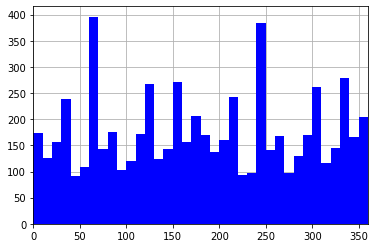
\includegraphics[height=0.55\textwidth]{images/5_emp_bebidas/street_network_analysis/histogram_cumbica.png}
    \end{subfigure}
    \begin{subfigure}{.49\textwidth}
      \raggedright
      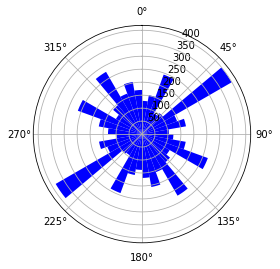
\includegraphics[height=0.55\textwidth]{images/5_emp_bebidas/street_network_analysis/polar_plot_cumbica.png}
    \end{subfigure}
    \caption*{\ Fonte: Produzido pelos autores Fernandes \& Alves}
\end{figure}

\subsection{Aprofundamento das análises de malha viária} \label{sec:aprofund-LMR}

Os métodos disponibilizados pelo pacote \textit{OSMnx} fornecem resultados que enriquecem o valor da pesquisa atual uma vez que é capaz de gerar uma série de estatísticas descritivas sobre diferentes malhas viárias.
Contudo, além da redundância de alguns dos parâmetros, também faz parte das limitações enfrentadas a falta de algumas variáveis mais detalhadas, como seria o caso de variáveis para traduzir em números os histogramas de orientação vistos anteriormente.
Sendo assim, é proposto um conjunto de novos parâmetros para quantificar malhas além dos que estão disponíveis nas configurações padrões do pacote \textit{OSMnx}, parâmetros estes que serão descritos a seguir.

Para começar o processo de quantificar o problema de orientação visto anteriormente, será interessante medir o grau de regularidade da distribuição de orientações apresentada pela malha.
Para tanto, defini-se uma distribuição uniforme de área equivalente à distribuição provinda da malha. 
Essa distribuição significaria o caso hipotético em que as vias estão uniformemente distribuídas em todas as direções possíveis.
Á partir daí é possível comparar a distribuição apresentada pela malha com a distribuição idealizada uniformemente, como ilustrada pela Figura \ref{fig:uniform_histogram}. 
%
A técnica adotada consiste em somar o quadrado da diferença de valores apresentados por essas duas distribuições em cada uma das direções.
Deste modo, cria-se uma medida que ``penaliza'' distorções muito grandes, as quais representariam uma malha onde as vias se concentram sempre em uma única direção específica.

\begin{figure}[htbp]
    \centering
    \caption{Exemplo de comparação entre distribuição real de orientações de vias e hipotética distribuição uniforme equivalente}
    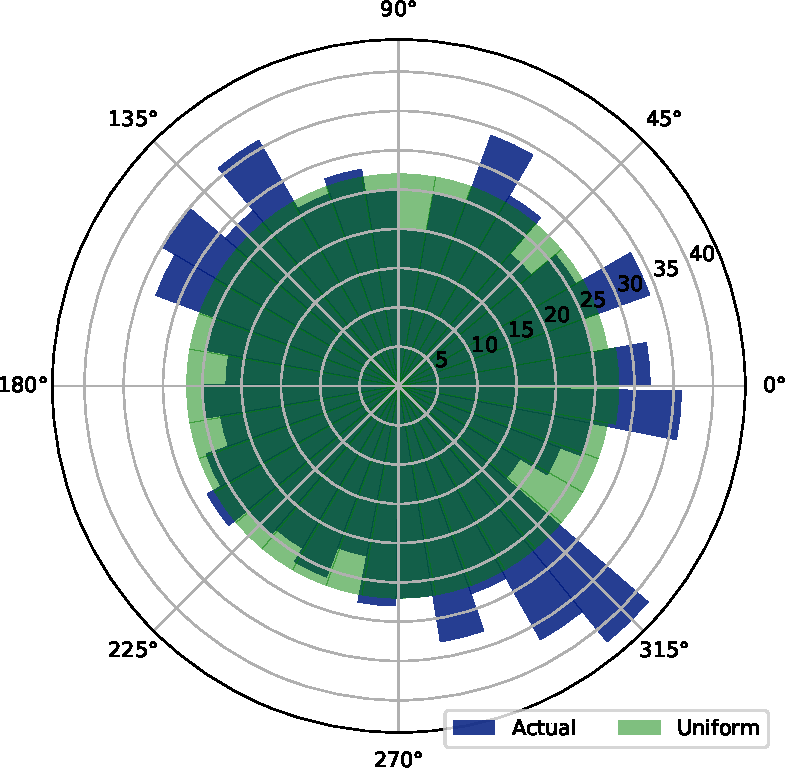
\includegraphics[height=0.45\textwidth]{images/4_materiais/lmr_analyzer/histogram_uniform.pdf}
    \caption*{Fonte: Produzido pelos autores Fernandes \& Alves}
    \label{fig:uniform_histogram}
\end{figure}

Ainda tomando como base o estudo de distribuições, é possível definir os parâmetros de \textit{skew} e \textit{kurtosis}, os quais representam o formato da distribuição analisada.
A variável \textit{skew} quantifica a simetria da distribuição, enquanto que a variável \textit{kurtosis} mede o quanto que a distribuição se aproxima de uma distribuição normal.
Ainda que nos casos estudados muitas vezes a distribuição não será aparente com uma distribuição normal, manter sob observação a variável \textit{kustosis} pode ser relevante para se estabelecer algumas confirmações.

Ademais, defini-se outras variáveis como, por exemplo, a média aritmética das direções e o intervalo de direção dominante.
%
Uma consideração importante sobre estas operações é que, para evitar resultados redundantes em termos de direção, é feita a conversão temporária do intervalo de direções, passando de 0º-360º para 0º-180º.
Este procedimento garante que o modelo não aponte, por exemplo, que a direção dominante e a segunda direção dominante sejam as iguais (porém de sentidos diferentes, e.g. 0º e 180º).
%
As variáveis propostas estão listadas a seguir:

\begin{itemize}
    \item \textit{\textbf{dominant\_direction}}: Intervalo de direção predominante, geralmente aberto limite superior e fechado no inferior. É a moda da distribuição de orientações analisada e pode variar de 0º a 180º.
    \item \textit{\textbf{dominant\_percentage}}: Porcentagem de arcos que pertencem ao intervalo de direções dominante dividido pelo total de arcos.
    \item \textit{\textbf{second\_dominant\_direction}}: Segundo intervalo predominante de direções. Pode variar de 0º a 180º.
    \item \textit{\textbf{second\_dominant\_percentage}}: Porcentagem de arcos que pertencem ao segundo intervalo de direções dominante dividido pelo total de arcos.
    \item \textit{\textbf{mean}} and \textbf{\textit{std}}: Média e desvio padrão, para fins estatísticos apenas. Essas variáveis dificilmente terão valor significativo para representar as direções em questão.
    \item \textit{\textbf{quadratic\_sum\_deviation}}: Soma dos quadrados da diferença entre distribuição apresentada e distribuição uniforme equivalente em cada um dos intervalos. Sempre positivo. Quanto mais próximo de zero, mais a distribuição se aproxima de uma distribuição uniforme, ou seja, a malha tende a não ter nenhuma direção de preferência.
    \item \textit{\textbf{skew}}: Coeficiente de assimetria da distribuição. É calculado como sendo o triplo da diferença entre média e mediana, dividido sobre o desvio padrão da amostra.
    \item \textit{\textbf{kurtosis}}: Momento central de quarta ordem ou média elevada à quarta potência, dividido pela quarta potência do desvio padrão da distribuição. 
\end{itemize}

Ao final, é possível exportar todos os resultados obtidos para o formato apropriado. Em geral, arquivos de extensão \textit{.shp} e \textit{.csv}.

\subsection{Modelos adicionais empregados}

Por fim, é possível descrever alguns modelos extras que também foram importantes para o desenvolvimento e análises do trabalho, como por exemplo a definição do centro de gravidade, ou centroide, para cada rota.
Todos os modelos que serão apresentados estão também disponíveis na biblioteca \textit{lmr\_analyzer} e descritos na seção de apêndice \ref{sec:AppCodes}. 

Embora encontrem-se disponíveis na literatura diversos modelos robustos de como simplificar de forma inteligente uma rota de entregas a um ponto representativo (\citeauthoronline{daganzo1984distance}, \citeyear{daganzo1984distance}), optou-se por adotar simplesmente uma média aritmética das coordenadas geodésicas de todos os PDEs de cada rota, excluindo o(s) CD(s) para que não haja viés.
%
Sendo assim, para uma rota de \textit{n} paradas, em que a primeira quanto a última parada correspondem ao CD, define-se o centroide da rota conforme a equação \ref{eq:CG_rota}.
%
\begin{equation}\label{eq:CG_rota}
    C.G._{route} = \left[lat_{C.G.},\; lon_{C.G.}\right] = \left[\frac{\sum_{i=2}^{n-1} lat_{i}}{n-2},\; \frac{\sum_{i=2}^{n-1} lon_{i}}{n-2}\right]
\end{equation}

Outro dos modelos propostos foi o cálculo da distância entre a rota e o CD.
Estas distâncias podem variar significativamente durante as observações, vista que em geral um único CD é responsável por atender mais de uma cidade. 
%
Novamente, ao buscar metodologias especializadas na literatura, como a proposta por \citeonline{novaes2000continuous}, os autores se depararam com modelos sofisticados e muitas vezes custosos computacionalmente.
%
O que se optou, portanto, foi a simplificação de modo a se computar a distância euclidiana entre o centro de gravidade da rota, descrito pela equação \ref{eq:CG_rota}, e o CD correspondente à rota.
Esta medida já traz uma boa estimativa do quão distantes os PDEs estão do CD. 

Por fim, um dos aspectos relevantes de serem mencionados é com relação à compactação das rotas, que consiste em quantificar a disposição e harmonia espacial das rotas analisadas.
%
Seguindo uma ordem de facilidade, pode-se definir um primeiro indicador como sendo o ``retângulo limite'' (\textit{bounding box}), o qual representa simplesmente o o retângulo de menor área que contenha todos os pontos da rota (excluído o CD).
Para cada \textit{bounding box} é possível calcular a área e a razão de aspecto, de modo a entender o quão dispersos no espaço os pontos das rotas se encontram. 

Ademais, define-se também um método para cálculo de ``polígonos convexos envelopadores'' (\textit{convex hull polygon}).
Um polígono \textit{convex hull} é um polígono convexo e sem buracos que contém todos os pontos desejados porém com menor área possível.
A determinação de tais polígonos foi realizada com auxílio do módulo \textit{spatial} disponível na biblioteca de aplicações científicas para Python denominada \textit{scipy} (\citeauthoronline{2020SciPy-NMeth}, \citeyear{2020SciPy-NMeth}).
A área do polígono \textit{convex hull} será o principal resultado a ser utilizado na análise, porém as coordenadas do polígono também podem ser obtidas, caso necessário.
%
Por outro lado, a evolução natural dos últimos dois métodos é o cálculo do ``retângulo rotacionado de mínima área'' (\textit{minimum rotated rectangule}) que, como o próprio nome diz, representará o retângulo de menor área que contenha todos os pontos da rota, porém sem a limitação anterior (\textit{bounding box}) de o retângulo estar fixado em uma rotação específica.

A titulo de observação, também foram estudados outros formatos não retangulares para estudo de compactação das rotas, como apresentado por \citeonline{gartner1998smallest}, porém a facilidade de implementação configurou-se como um critério importante para seleção do modelo e, desta forma, optou-se pelo método do \textit{minimum rotated rectangule}.

Finalmente, um resumo das medidas que serão calculadas conforme apresentado nesta subseção estão disponíveis logo abaixo:
\begin{itemize}
    \item \textbf{\textit{centroid\_mean}}: Média das coordenadas latitude e longitude dos PDEs presentes na rota.
    \item \textbf{\textit{centroid\_std}}: Desvião padrão das coordenadas latitude e longitude dos PDEs presentes na rota. 
    \item \textbf{\textit{bbox}}: Conjunto de quatro coordenadas definindo o \textit{bounding box} dos pontos da rota, sendo eles: latitude máxima e mínima e longitude máxima e mínima. 
    \item \textbf{\textit{bbox\_area}}: Área do retângulo definido pelo \textit{bounding box}.
    \item \textbf{\textit{bbox\_aspect\_ratio}}: Razão de aspecto do \textit{bounding box}, definida como a divisão do lado maior pelo lado menor.
    \item \textbf{\textit{convex\_hull\_coords}}: Coordenadas do polígono \textit{convex hull} que contém todos os pontos da rota, com exceção do CD.
    \item \textbf{\textit{convex\_hull\_polygon\_area}}: Área do polígono \textit{convex hull}.
    \item \textbf{\textit{mrr}}: Retângulo rotacionado de mínima área e que contenha todos os pontos da rota. É calculado com base no atributo \textit{convex\_hull\_coords}. 
    \item \textbf{\textit{mrr\_area}}: Área do retângulo rotacionado de mínima área.
    \item \textbf{\textit{mrr\_aspect\_ratio}}: A razão de aspecto do retângulo rotacionado de mínima área.
\end{itemize}

Quaisquer outros métodos que venham a ser utilizados para obtenção dos resultados serão explicados pontual e brevemente, porém, finaliza-se este Capítulo tendo sido descritas as metodologias que foram elaboradas ao longo do trabalho com auxílio das referências citar, bem como as hipóteses simplificadoras de cada modelo. 
